\documentclass[11pt, wide]{article}
    
    \usepackage[utf8]{inputenc}
    \usepackage[OT4]{polski}
    
    \usepackage{graphicx}
    \usepackage{caption}
    \usepackage{subcaption}
    \usepackage{epstopdf}
    
    \usepackage{hyperref}
    \usepackage{url}
    \usepackage{bbm}
    \usepackage{comment}
    \usepackage{makecell}
    \usepackage{xcolor}
    \usepackage{listings}
    \usepackage{secdot}


    \date{Wrocław, \today}
    \title{Łukasz Klasiński\\\LARGE\textbf{Model konceptualny projektu z \\Baz Danych\\}
    Prowadzący : Jan Otop}
    \begin{document}
    \maketitle
    \thispagestyle{empty}
    \section{Diagram E-R }
    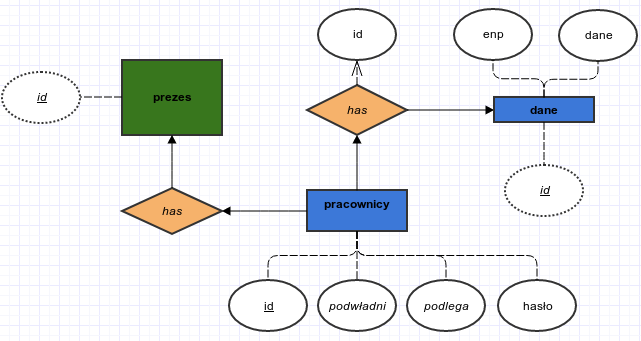
\includegraphics[width=\textwidth]{er}    

    Diagram pokazuje koncept bazy dla danego problemu. Atrybut \textit{podwładni}
    ze zbioru \textbf{pracownicy}, oznaczaja wszystkich bezpośrednio podległych pracowników. Z kolei
    \textit{podlega} pracowników, którym bezpośrednio lub pośrednio podlega. 
    Encja \textbf{prezes} zawiera pojedyńczy wpis, zawierający \textit{id} pracownika, który
    jest prezesem.\\

    Użytkownik \textbf{\textit{app}} ma możliwość odczytu oraz zapisu encji pokolorowanych
    na niebiesko. Z kolei \textbf{\textit{init}} ma dostęp do całej bazy danych.

    \section{Implemetacja}
    Funkcje dodające/modyfikujące użytkowników będą wykonywać standardowe
    funkcje \textit{SELECT} oraz \textit{UPDATE} języka sql, ze sprawdzaniem, czy 
    dany użytkownik posiada odpowiednie prawa.\\    
    Funkcje szukające pracowników, którym dana osoba podlega będą zwracać wartości zawarte w liście \textit{podlega}. 
    Z kolei przy szukaniu podległych pracowników, rekurencyjnie będą zwracane wartości \textit{podwładni}.
    \\Podobnie usuwanie pracownika, będzie rekurencyjnie usuwać dane kolejnych pracowników.
    \\Tworzenie wpisu prezesa dodatkowo doda odpowiedni wpis do tabeli o tej nazwie.


\end{document}

